\documentclass[11pt]{article}

\usepackage{geometry}
\geometry{letterpaper, margin=1in}
\usepackage{graphicx}
\usepackage{booktabs}
\usepackage{longtable}
\usepackage{amsmath}
\usepackage{microtype}
\usepackage{xcolor}
\usepackage{caption}
\usepackage{float}
\usepackage{enumitem}
\usepackage{tabularx}
\usepackage{array}
\usepackage[hidelinks]{hyperref}

\captionsetup{font=small, labelfont=bf}
\newcommand{\code}[1]{\texttt{#1}}
\newcommand{\todo}[1]{\textcolor{red}{[#1]}}
\setlength{\tabcolsep}{4pt}
\renewcommand{\arraystretch}{1.12}

\title{\vspace{-2.2em}\bfseries Recursive self-improvement, gated by evidence\\[0.3em]
\large An engine that lets deployed agents improve their own operation --- proposing, proving, canarying and shipping their own corrections --- measured where the world changes under a long-running agent and outcome learning alone cannot recover}

\author{SenseLab Research\\[0.3em]\normalsize\url{https://sense-lab.ai}}
\date{Preprint v0.2 --- development seeds --- September 2026}

\begin{document}
\sloppy
\maketitle

\begin{abstract}
\noindent
Agents that run for months on complex work face a problem no static model solves: the world
they operate in changes under them, their tasks never repeat exactly, and every session that
acts on what used to be true fails the same way until something in the system changes. Scaling
such agents is not a retrieval problem. It is a self-improvement problem: the system must detect
that its own knowledge has gone wrong, propose a correction, prove it, release it safely, learn
from the result, and do all of this without a person in every loop and without shipping the
wrong thing to every agent at once. SenseLab is a recursive self-improvement engine built for
that. Outcome evidence changes what agents act on (level~0); a repair agent drafts corrections
that must pass a stand-in replay, the customer's own replay and a live canary that shows them
no worse than the rule they replace before they ship, reversibly (level~1); the loop's own history feeds its next draft
(level~2); and the record it produces trains the next model and the repair prompt itself
(level~3). This paper is the first measurement of such a loop. We evaluate the whole engine ---
never its parts against each other --- on a continual benchmark in which the correct action for
a task class changes \emph{conditionally} at episode 30 of 100, so that half of the class needs
the new rule and half still needs the old one, and no amount of retrying the old action can
recover the first attempt. On the development seeds SenseLab takes the new action first in
33\,\% of moved-half episodes against 5--19\,\% for a frontier model alone and three vector-store
baselines, holding unchanged work at 96\,\%; a context window carrying every prior note reaches
the same 33\,\% at 1.5$\times$ the all-in cost (2.1$\times$ the agent's own). Level~1 has not yet added to level~0 on these seeds, and the
tables say why: no canary has decided inside a 100-episode cell, nor in 200 with ten agents ---
where one reaches its floor the failure has already stopped recurring in control, so there is
nothing live to gate --- and until the last engine cuts what the proof tiers passed was the
unconditional rule --- on the current cut the proof rejects 15 of
17 regime fixes, and the two it passes are a wholesale flip and a retry ladder, neither of which
states the condition the world changed on. The paper's main contribution is the record of how a
preregistered benchmark found eleven things about the loop's evidence path --- nine defects, all
fixed in production between runs and re-measured on the same protocol --- and what each
says about building self-improving systems that can be trusted: what counts as a regime shift,
how a situation is identified, what a fix must be proved against, who grades the proof, what
counts as traffic, and which runs a canary can grade. Every number here is from development seeds; the confirmatory seeds run once,
after the analysis is frozen.
\end{abstract}

\section{Introduction}

The hard problem in scaling agents is not capability but longevity. A model that solves a task
today is deployed into an operation that runs for months: the policies it applies are rewritten,
the dependencies it pins are audited, the workflows it follows are changed by people who never
tell it. Its tasks never repeat exactly, so nothing can be memorised; and the failure that
matters is not that it cannot find what it knows but that it acts, confidently, on what
\emph{used} to be true --- and will do so again on every session that reads the same thing,
until something in the system changes. A static model with a static context degrades
monotonically in such a world. A person in every loop does not scale.

The path forward is a system that improves its own operation from its own results, and whose
improvements compound: recursive self-improvement. It is also the thing everyone is right to be
nervous about. A self-modifying system amplifies its own errors as readily as its corrections;
a model that drafts fixes from failure evidence will draft wrong ones, and a wrong fix written
into what every agent reads damages every session at once. The question is therefore not whether
deployed agents should improve themselves --- at scale there is no alternative --- but what
discipline makes it safe enough to run in production: evidence before proposal, proof before
release, staged exposure before full exposure, reversibility after, and an audit trail
throughout.

SenseLab is an engine built on that discipline, and this paper measures it. Its loop has four
levels (\S\ref{sec:engine}). At level~0, every session's outcome is attributed to exactly what
the agent read and did, and that evidence --- validated, contested, discredited --- changes what
the next session acts on. At level~1, an entry that was validated and now fails is a
\emph{regime shift}; a repair agent drafts a correction on a branch with a manifest of the runs
it claims to repair and must not break, and the correction must pass a stand-in replay (Tier~1),
the customer's own agent replaying the case set (Tier~2) and a live canary on a hashed share of
sessions that must show the fix no worse than the rule it replaces (Tier~3) before it ships ---
reversibly. At level~2, the loop's
own history (what it tried on this entry, what passed, what regressed) is evidence for its next
draft. At level~3, the record the loop produces trains the next model and the repair prompt
itself. The claim is not that the repair agent is clever. The claim is that \textbf{a correction
may only change behaviour after it has been tested on the runs it claims to repair and shown
no worse than the control arm on live traffic}, and that a system built this way recovers faster than
one that can only demote what failed, while shipping fewer wrong corrections than one that ships
on a passed test.

We ask, on a benchmark that knows the true rule before and after every change, whether the
whole engine recovers faster and further than the frontier model alone, than three vector-store
baselines, than a context window carrying the cell's entire history, and than its own ablations;
whether it damages what still worked; what it ships; and what it costs. We call the whole system
\emph{SenseLab} throughout: the levels are not features to be compared against each other, they
are what the engine delivers, and the ablations that switch parts of it off appear in one
attribution table and nowhere else.

\paragraph{What this version is.} This is a development-seed report (seeds 11 and 23 of six),
written while the confirmatory seeds are still to run. It exists because the preregistration
(\S\ref{sec:prereg}) committed to reporting every prediction, met or falsified, and most of the
predictions so far were falsified --- by defects in the loop's evidence path that the benchmark
found and that were fixed in production between runs. Section~\ref{sec:findings} is the record
of that, and we think it is the paper's main contribution: a self-improving system is only as
trustworthy as its evidence path, and every one of these defects would have been invisible to
a benchmark that measured retrieval. The headline tables (\S\ref{sec:results}) are the state of
the engine on its current cut; the confirmatory numbers will differ, and the direction they
differ in is itself predicted (\S\ref{sec:pending}).

\section{The engine under test}
\label{sec:engine}

Everything measured is production code on the SenseLab SaaS, run against a dedicated Enterprise
account; no constant below was tuned for this study, and each is quoted from the deployed source.
The harness never decides anything: it seals sessions through the public API, and the loop's own
scheduler proposes, tests, gates and ships. The four levels of the loop, in the order evidence
flows through them:

\paragraph{Level 0 --- outcome learning: the evidence record.} An agent calls \code{briefing} and \code{retrieve}
before acting, \code{record\_action} and \code{record\_attempt} as it goes, and
\code{commit\_outcome} when the task ends. The sealed trace carries the exact read set; the
outcome is attributed to it (an entry read by a run that failed after a recorded attempt against
it is charged the failure; an entry read by a clean success is credited). Entries carry an
\emph{evidence status} --- \code{untested}, \code{validated}, \code{contested},
\code{discredited} --- and \code{retrieve} returns, with the hits, per-action priors
(won/lost here on similar tasks) and a recommendation mode: \code{act}, \code{explore} (assigned
per agent, so peers explore different actions) or \code{escalate}. That is level~0 alone; it is the row
``SenseLab $-$ repair loop'' in Table~\ref{tab:attribution}.

\paragraph{Regime shift and situation.} A \emph{regime shift} is an entry validated at least three
times that now fails: a sealed failure whose read set contains such an entry, or a recorded failed
attempt against it. A shift is not a first-exposure failure --- an entry that was never validated
cannot have shifted --- and the guard that separates the two was the third defect this study found
(\S\ref{sec:findings}). Because the same entry can be right in one situation and wrong in another,
the agent labels each session with an \code{attributes.situation}, and the service resolves the
label to the agent's canonical situation (a stemmed-token rule, Jaccard $\geq 0.5$, with an
embedding second stage at cosine $\geq 0.75$); the shift, the proof set and the canary are all
scoped to the situation. A shift proposes a fix automatically (\code{auto\_propose}, per agent).

\paragraph{Level 1 --- the repair loop. Proposal.} The repair agent (GPT-5-class, 50k-token budget) reads the failing runs,
the entry, and the loop's own history on that entry, and writes a corrective entry (lever
\code{knowledge}) or a conditional procedure with conditions, steps and a verify (lever
\code{procedure}) on memory branch \code{repair/<fix>}, with a \emph{manifest}: the runs it
predicts it repairs, the runs it must not break, and an expected prevention (0.5 by default). A
\code{code} lever is handed off and never auto-shipped.

\paragraph{Tier 1 --- stand-in replay.} A stand-in model re-runs each manifest case with the
branch as memory and tool calls answered from the recorded run; fidelity is the share of steps
answered from the record, and a test below the agent's fidelity floor (0.5) does not count as a
pass. A test can be \code{passed}, \code{failed} or \code{inconclusive}.

\paragraph{Tier 2 --- customer replay.} The fix's \emph{case set} --- HMAC-signed cases --- is
delivered to the customer's agent, which re-runs them on the branch and seals the results; the
service grades each replay against the case's expectation. For a regime fix the case set is the
run the shift fired on, up to three more of the situation's failed runs (the shift; the fix must
turn them into successes) and up to three of its passed runs (what still works; the fix must not
break them). A case no judge graded is graded on the outcome the replay reports, and --- since
the last cut --- on its attempts: a success reached \emph{after a recorded failed attempt} fails
the case (\S\ref{sec:findings}, finding 9).

\paragraph{Tier 3 --- canary.} A passed fix opens a canary: sessions are bucketed by
$\mathrm{sha256}(\mathit{fix}{:}\mathit{session})$, a share \code{pct} reads from the branch,
writes always go to \code{main}, and the trace is stamped with its branch. \code{decide()}
requires both arms to reach \code{min\_outcomes} graded runs --- runs \emph{in the fix's
situation or that read an entry the fix is about} (cut \emph{post-canary-ni}; before it,
situation only: \S\ref{sec:findings}, finding 11) --- and guards that the canary's success rate
is not below the control's. The canary is the loop's \emph{harm} gate: the replay tiers prove
the benefit on the failing runs, and live traffic has to show the change does not make the agent
worse on the runs the old rule still served. It passes when the canary arm recurs significantly
less (one-sided two-proportion $z$-test, $p<0.05$) or when the one-sided 95\,\% upper bound
(Newcombe) on canary$-$control recurrence is under a margin of 10 points with the failure live in
control; it fails when the canary arm recurs significantly more. Before \emph{post-canary-ni}
the primary asked for a significant improvement, and no canary ever passed (finding 11). The
benchmark maps the production defaults (10\,\%, 20 outcomes, 14 days) to \code{pct}=50,
\code{min\_outcomes}=8, a timeout of 60 sessions (the cell horizon --- 100 or 200 --- from
amendment~(v) on), evaluated every 5 graded sessions. One canary per agent at a time.

\paragraph{Ship, verify, revert.} Policy \code{auto\_after\_canary} merges a passed canary's branch
into \code{main}; \code{auto\_after\_replay} (the ``$-$ canary'' ablation) merges on a passed
Tier~2. A feedback contract holds a fix if fewer than 80\,\% of recent traces carry provenance.
Prevention is verified over the following window; a regressed fix is rolled back, restoring the
pre-fix versions. Continuous judges (a two-tier \code{gpt-5-mini}$\to$\code{gpt-5} rubric pack)
grade sealed traffic and open incidents that are the second producer of proposals.

\paragraph{Level 2 --- the loop reads its own history.} Every fix event on an entry --- proposed,
tested, replayed, shipped, regressed, rolled back --- is written back as evidence on that entry,
and the repair agent's next draft on the same entry reads it: what was tried, what passed, what
regressed. A loop that cannot see its own record repeats its own mistakes; this one is measured
on whether it stops (the two-change protocol of the flagship experiment, not yet run).

\paragraph{Level 3 --- the record trains the model and the improver.} The traces the loop
produces --- including the repair trajectories and the cases it pinned --- are a training set:
Managed Models (\code{senselab-s1}) are distilled from them and served with the same evidence
record as their memory (\S\ref{sec:results}); and the repair prompt itself is A/B tested across
proposals, with proven fixes per prompt as the score, which is the improver improving itself.
Only the first rung of the first of these is measured in this version.

\section{Benchmark and protocol}
\label{sec:prereg}

\paragraph{Preregistration.} Hypotheses, arms, metrics, seeds, the dev/confirmatory split and the
analysis freeze were registered before the first run (\code{HYPOTHESIS\_RSI.md}, tag
\code{prereg-rsi-v1}); every change since is a dated amendment (a)--(x) appended below the
original, each with a prediction and what would falsify it. Seeds 11 and 23 are the development
seeds; 37, 41, 59 and 73 run once, after the analysis code is tagged \code{analysis-freeze-rsi}.
Engine changes made between runs are recorded with their deploy cut to the second, and every
result carries the engine cut as a covariate.

\paragraph{Environment.} Two families of the ten in the benchmark, both with tool-using agents and
oracle-graded outcomes: \code{support} (a helpdesk agent with account, order and export tools;
15 issue classes) and \code{ci-fix} (an agent repairing failing CI on a repository; 10 failure
classes). Every task instance is generated, never repeated, with random identifiers
(\code{opaque\_ids}) so nothing can be read off an id. 100 episodes per cell, 300 distractor
entries in every store, retry budget 3, one agent identity per cell, GPT-5.5 at low effort, a
post-episode reflection note in every arm that has a store.

\paragraph{Change set C.} At episode 30 a subset of classes changes \emph{conditionally}: the
correct action moves for instances with one attribute value (the \emph{moved half}) and stays for
the others (the \emph{kept half}). Half of post-change tasks are drawn from changed classes. Set C
was written after the pilots showed that on an unconditional change (set A) outcome learning
alone recovers nearly everything a maintainer who knew the rule would (\S\ref{sec:findings},
finding 4): the only place a written rule can beat demotion is where demotion has no signal to
demote --- the entry is still right half the time. Set C is registered by hash; its remaining
eight families are written blind before the confirmatory run.

\paragraph{Systems.} Frontier alone (no store); context window (every prior note and outcome of
the cell in the prompt, most recent first, 24k tokens); pgvector (bge-small, cosine top-5 over
notes); pgvector + rerank (the same cross-encoder SenseLab serves); pgvector + outcomes (notes,
LLM consolidation every 5 episodes, a per-entry win/loss counter shown to the agent); and SenseLab
(\S\ref{sec:engine}, policy \code{auto\_after\_canary}). Mem0 and Zep are not run (an earlier
grid covers them~\cite{senselab-cl}). The ablations --- SenseLab $-$ canary
(\code{auto\_after\_replay}) and SenseLab $-$ repair loop (policy \code{review}, proposals never
approved) --- appear in Table~\ref{tab:attribution} only.

\paragraph{Endpoints.} First-attempt success on the moved half after the change (primary);
first-attempt success on the kept half and on unchanged classes (collateral damage); episode
success and escalation; the fix lifecycle (proposed, Tier~1, Tier~2, canary, shipped, reverted);
and cost. Infra errors are excluded from rates and reported. Intervals are cell-level bootstrap
(2,000 resamples). With four cells per system on development seeds these intervals are wide by
construction and are shown so that no reader mistakes a dev-seed difference for a result.

\section{Results on the development seeds}
\label{sec:results}

\subsection{After the rule changes conditionally}

\begin{table}[H]
\centering\scriptsize\setlength{\tabcolsep}{3pt}
\resizebox{\linewidth}{!}{\begin{tabular}{lrrrrrrr}
\toprule
\textbf{system} & \textbf{moved half} & \textbf{kept half} & \textbf{unchanged classes} & \textbf{pre-change} & \textbf{episode success} & \textbf{escalated} & \textbf{\$/ep} \\
\midrule
Frontier alone & 17 \% (13/75) [0, 41] & 38 \% (25/65) [11, 78] & 66 \% (93/140) & 61 \% (73/120) & 84 \% (334/400) & 16 \% (66/400) & 0.011 \\
Context window & 33 \% (25/75) [0, 78] & 98 \% (64/65) [94, 100] & 100 \% (140/140) & 85 \% (102/120) & 92 \% (366/400) & 8 \% (34/400) & 0.070 \\
pgvector & 17 \% (13/75) [2, 38] & 45 \% (29/65) [13, 78] & 93 \% (130/140) & 71 \% (85/120) & 88 \% (353/400) & 12 \% (47/400) & 0.027 \\
pgvector + rerank & 5 \% (4/75) [1, 9] & 86 \% (56/65) [78, 95] & 94 \% (132/140) & 79 \% (95/120) & 90 \% (359/400) & 10 \% (41/400) & 0.028 \\
pgvector + outcomes (DIY) & 19 \% (14/75) [0, 44] & 55 \% (36/65) [39, 78] & 80 \% (112/140) & 70 \% (84/120) & 88 \% (351/400) & 12 \% (49/400) & 0.035 \\
SenseLab & 33 \% (25/75) [14, 56] & 63 \% (41/65) [40, 76] & 96 \% (134/140) & 81 \% (97/120) & 92 \% (368/400) & 8 \% (32/400) & 0.033 \\
\bottomrule
\end{tabular}}
\caption{After the rule changes conditionally (set C, change at episode 30 of 100; GPT-5.5; four cells per system: \code{support} and \code{ci-fix} $\times$ seeds 11 / 23). First-attempt success on every post-change episode. \emph{Moved half}: changed-class instances whose rule changed; \emph{kept half}: changed-class instances whose rule did not. Brackets: cell-level bootstrap 95\% interval. Development seeds; SenseLab on the \code{post-canary-ni} engine cut.}
\label{tab:headline}
\end{table}



\begin{figure}[H]
\centering
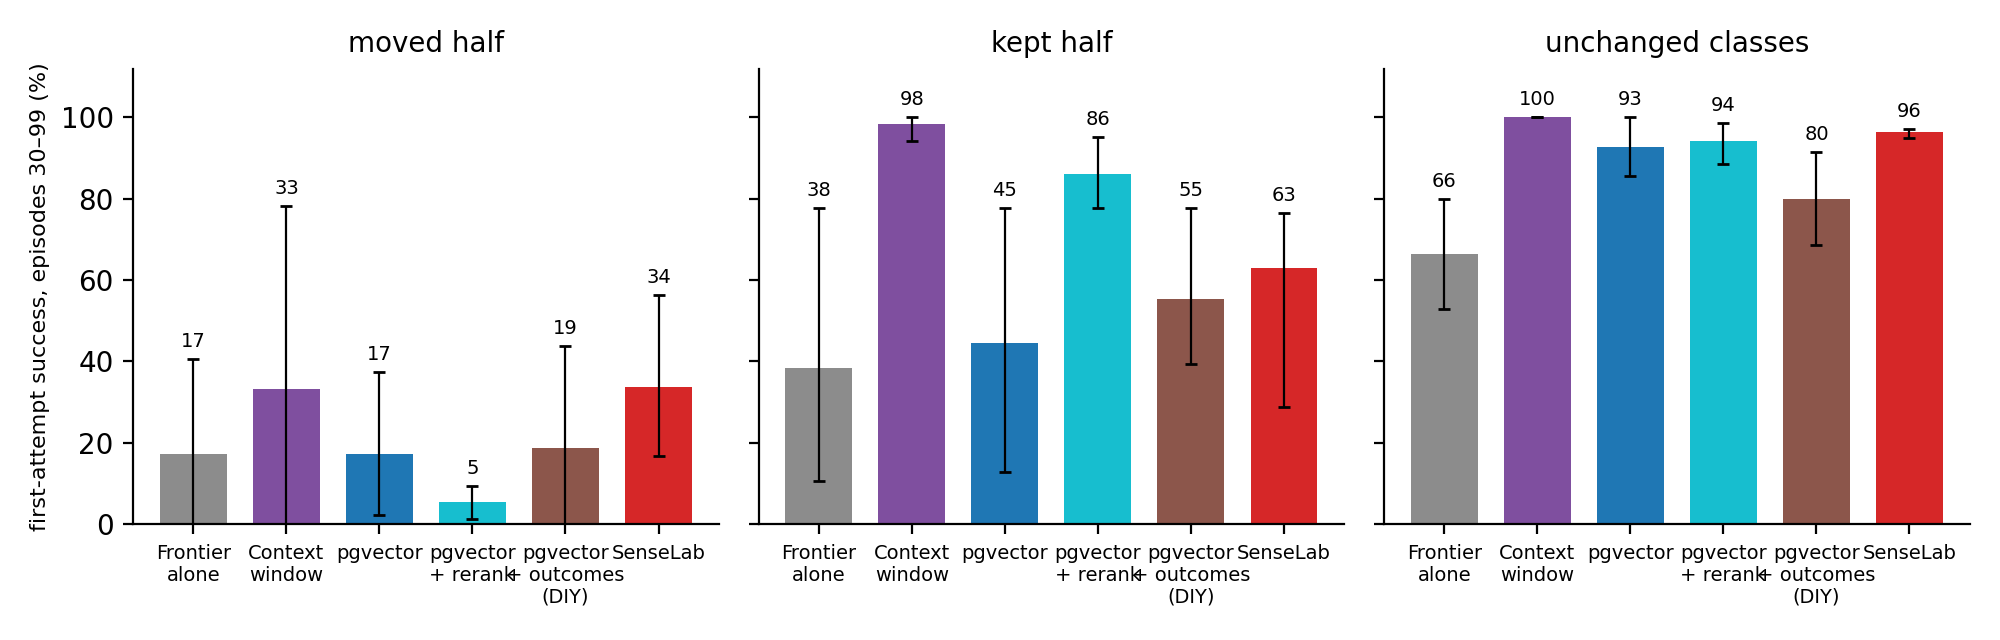
\includegraphics[width=\textwidth]{figures/fig_headline.png}
\caption{First-attempt success after the rule changes conditionally (episodes 30--99, four cells,
GPT-5.5): the moved half, the kept half and the unchanged classes, one bar per system, with
cell-level bootstrap 95\,\% intervals. Same numbers as Table~\ref{tab:headline}.}
\label{fig:headline}
\end{figure}

Table~\ref{tab:headline} is the state of the engine on its current cut, \code{post-canary-ni}
(\S\ref{sec:findings}, findings 8--11 live). Three things
are in it. First, on the moved half every retrieval memory is at or below the frontier model
alone: a note that says ``do $X$ for class $C$'' is retrieved as confidently after the change as
before, and pgvector with reranking --- the best retriever --- is the \emph{worst} system on the
moved half at 5\,\%, because it retrieves the stale note most reliably. Second, SenseLab is the
only system that recovers the moved half on both families while holding the unchanged classes
at 96\,\%: 33\,\% [14, 56] against 5--19\,\% for the frontier model and the three vector stores,
winning every paired cell. The context window ties it exactly (33\,\%) by beating it on
\code{ci-fix} (78 against 56: the whole history fits in 24k tokens and the model can see the
change happen) and doing nothing on \code{support} (0/43, SenseLab 7/43), at 1.5$\times$ the all-in cost
(2.1$\times$ the agent's own calls) and 3.7$\times$ the tokens. Third, SenseLab pays on the kept half: 63\,\% against 86\,\% and 98\,\% for the two
systems that keep applying the old rule most reliably (pgvector + rerank and the context window). That cost is the shape of the mechanism --- the entry is
marked contested and the agent explores where the old action was still right --- and it is the
number the repair loop exists to remove: a written conditional rule would recover the moved half
\emph{without} giving up the kept one. Whether it does yet is Table~\ref{tab:attribution}.

\begin{table}[H]
\centering\scriptsize\setlength{\tabcolsep}{3pt}
\resizebox{\linewidth}{!}{\begin{tabular}{lrrrrrrrr}
\toprule
\textbf{pair} & \textbf{support s11} & \textbf{support s23} & \textbf{ci-fix s11} & \textbf{ci-fix s23} & \textbf{mean} & \textbf{cells won} & \textbf{p} & \textbf{p (Holm)} \\
\midrule
SenseLab $-$ Frontier alone & +26 & +5 & +11 & +23 & +16 & 4/4 & 0.125 & 0.625 \\
SenseLab $-$ Context window & +26 & +5 & -26 & -15 & -3 & 2/4 & 0.875 & 0.875 \\
SenseLab $-$ pgvector & +22 & +5 & +11 & +31 & +17 & 4/4 & 0.125 & 0.625 \\
SenseLab $-$ pgvector + rerank & +22 & +5 & +47 & +46 & +30 & 4/4 & 0.125 & 0.625 \\
SenseLab $-$ pgvector + outcomes (DIY) & +26 & +5 & +5 & +23 & +15 & 4/4 & 0.125 & 0.625 \\
\bottomrule
\end{tabular}}
\caption{SenseLab minus each system on the moved half, per cell, in percentage points, paired on (family, seed).}
\label{tab:paired}
\end{table}


\begin{table}[H]
\centering\scriptsize\setlength{\tabcolsep}{3pt}
\resizebox{\linewidth}{!}{\begin{tabular}{lrrrrrr}
\toprule
\textbf{system} & \textbf{support: moved} & \textbf{support: kept} & \textbf{support: unchanged} & \textbf{ci-fix: moved} & \textbf{ci-fix: kept} & \textbf{ci-fix: unchanged} \\
\midrule
Frontier alone & 0 \% (0/43) & 78 \% (21/27) & 53 \% (37/70) & 41 \% (13/32) & 11 \% (4/38) & 80 \% (56/70) \\
Context window & 0 \% (0/43) & 96 \% (26/27) & 100 \% (70/70) & 78 \% (25/32) & 100 \% (38/38) & 100 \% (70/70) \\
pgvector & 2 \% (1/43) & 78 \% (21/27) & 86 \% (60/70) & 38 \% (12/32) & 21 \% (8/38) & 100 \% (70/70) \\
pgvector + rerank & 2 \% (1/43) & 78 \% (21/27) & 90 \% (63/70) & 9 \% (3/32) & 92 \% (35/38) & 99 \% (69/70) \\
pgvector + outcomes (DIY) & 0 \% (0/43) & 78 \% (21/27) & 69 \% (48/70) & 44 \% (14/32) & 39 \% (15/38) & 91 \% (64/70) \\
SenseLab & 16 \% (7/43) & 44 \% (12/27) & 96 \% (67/70) & 56 \% (18/32) & 76 \% (29/38) & 96 \% (67/70) \\
\bottomrule
\end{tabular}}
\caption{By family: first-attempt success on the moved half, the kept half and the unchanged classes.}
\label{tab:byfamily}
\end{table}



\begin{figure}[H]
\centering
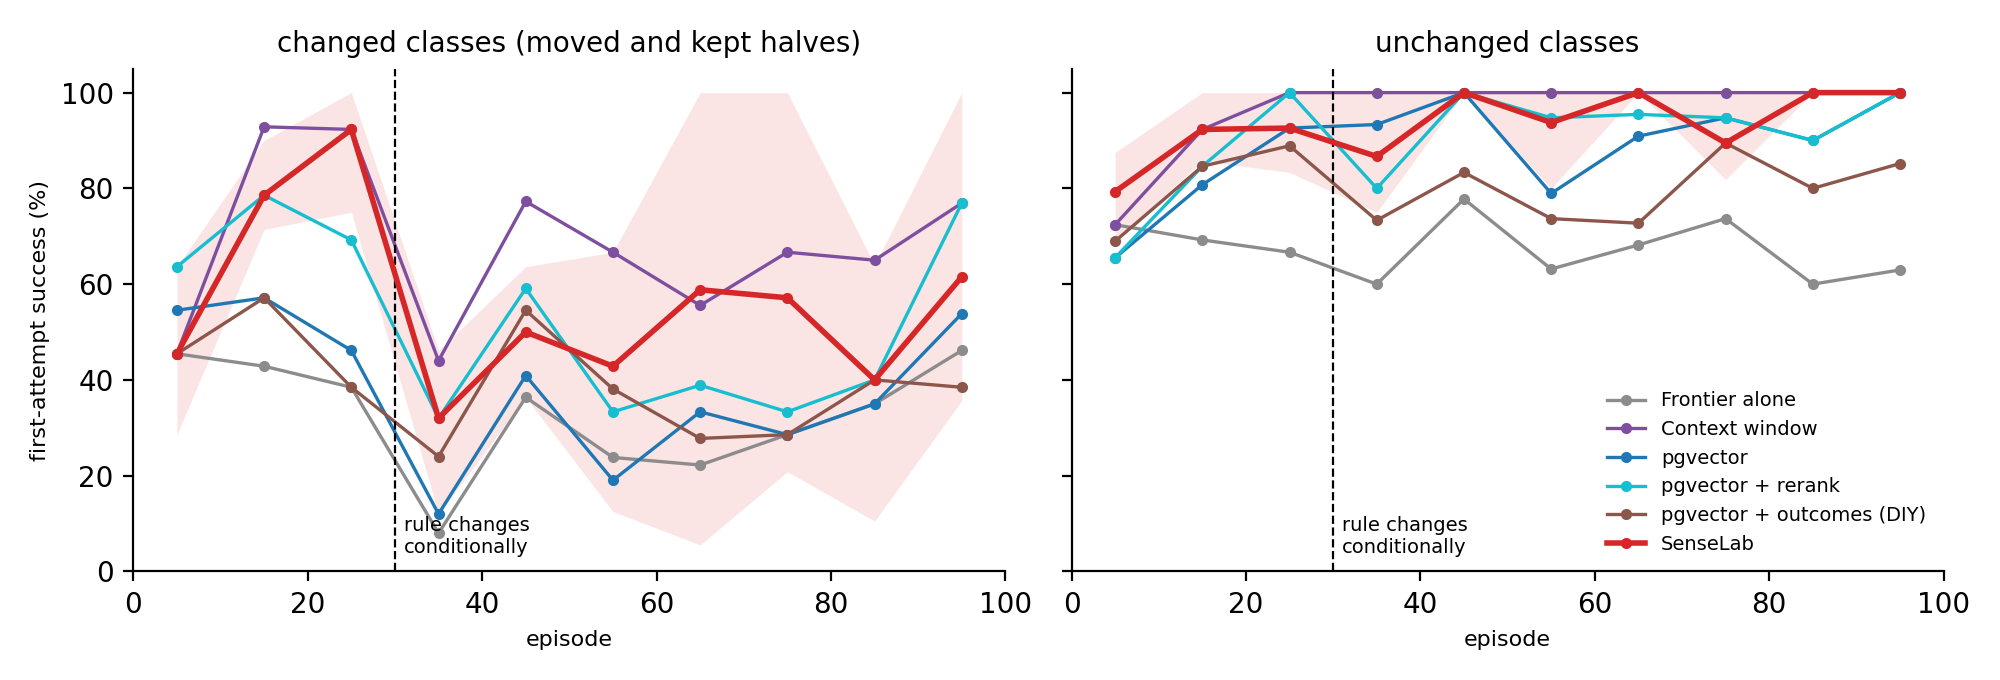
\includegraphics[width=\textwidth]{figures/fig_curves.png}
\caption{First-attempt success by 10-episode block across the change at episode 30, pooled over
the four cells: the classes whose rule changes (left; before the change every system is at
80--90\,\%, after it the rule holds for the kept half only) and the unchanged classes (right).
SenseLab is drawn heavy with its cell-level bootstrap band; the other systems' bands are of the
same width and are omitted for legibility. Recovery is partial for every system inside 70
episodes; the context window recovers most on \code{ci-fix} because the whole history fits in
its prompt (Table~\ref{tab:byfamily}).}
\label{fig:curves}
\end{figure}

\subsection{Attribution: what level 1 adds to level 0, so far}

\begin{table}[H]
\centering\scriptsize\setlength{\tabcolsep}{3pt}
\resizebox{\linewidth}{!}{\begin{tabular}{lrrrrrrrr}
\toprule
\textbf{system} & \textbf{moved half} & \textbf{kept half} & \textbf{unchanged classes} & \textbf{pre-change} & \textbf{episode success} & \textbf{escalated} & \textbf{infra err} & \textbf{\$/ep} \\
\midrule
SenseLab & 33 \% (25/75) [14, 56] & 63 \% (41/65) [40, 76] & 96 \% (134/140) & 81 \% (97/120) & 92 \% (368/400) & 8 \% (32/400) & 0 & 0.033 \\
SenseLab $-$ canary & 39 \% (29/75) [14, 66] & 62 \% (40/65) [42, 74] & 99 \% (139/140) & 79 \% (95/120) & 91 \% (365/400) & 9 \% (35/400) & 0 & 0.033 \\
SenseLab $-$ repair loop & 51 \% (38/75) [33, 73] & 69 \% (45/65) [58, 76] & 96 \% (135/140) & 81 \% (97/120) & 92 \% (369/400) & 8 \% (31/400) & 0 & 0.032 \\
\bottomrule
\end{tabular}}
\caption{Attribution. SenseLab against its own ablations on the same protocol: without the canary (policy \code{auto\_after\_replay}, same run) and without the repair loop (policy \code{review}: proposals never approved; outcome learning alone). This is the only table in which the ablations appear.}
\label{tab:attribution}
\end{table}


On these seeds level~1 does not yet add to level~0. Without the repair loop (policy
\code{review}: the loop proposes, nothing ships, the memory learns from outcomes alone) the moved
half is 51\,\% and the kept half 69\,\%; with it, 33\,\% and 63\,\%; without the canary but with
the replay gate, 39\,\% and 62\,\%. The intervals overlap throughout and nothing here is a
difference. What the lifecycle table shows is \emph{why}, and it is not that the loop is idle.

\begin{table}[H]
\centering\scriptsize\setlength{\tabcolsep}{3pt}
\resizebox{\linewidth}{!}{\begin{tabular}{lrrrrrr}
\toprule
\textbf{arm} & \textbf{proposed} & \textbf{regime / judge} & \textbf{T1 pass / inc. / fail} & \textbf{T2 pass / fail / open} & \textbf{canaries run / undecided} & \textbf{shipped} \\
\midrule
SenseLab, pre-seam4 & 9 & 5 / 4 & 7 / 2 / 0 & 2 / 2 / 0 & 3 / 3 & 0 \\
SenseLab $-$ canary, pre-seam4 & 8 & 4 / 4 & 4 / 3 / 1 & 1 / 2 / 0 & 0 / 0 & 1 \\
SenseLab, post-seam5 & 16 & 12 / 4 & 5 / 10 / 1 & 6 / 3 / 7 & 4 / 3 & 0 \\
SenseLab $-$ canary, post-seam5 & 17 & 13 / 4 & 12 / 4 / 1 & 9 / 7 / 1 & 0 / 0 & 9 \\
SenseLab, post-seam5b & 24 & 19 / 5 & 14 / 9 / 1 & 15 / 8 / 1 & 6 / 4 & 0 \\
SenseLab $-$ canary, post-seam5b & 16 & 13 / 3 & 10 / 5 / 1 & 11 / 4 / 0 & 0 / 0 & 11 \\
SenseLab, post-clean-success & 16 & 13 / 3 & 9 / 7 / 0 & 3 / 13 / 0 & 3 / 3 & 0 \\
SenseLab $-$ canary, post-clean-success & 17 & 13 / 4 & 9 / 4 / 4 & 2 / 12 / 3 & 0 / 0 & 2 \\
SenseLab, post-canary-ni & 13 & 8 / 5 & 4 / 8 / 0 & 4 / 7 / 1 & 3 / 3 & 0 \\
SenseLab $-$ canary, post-canary-ni & 14 & 10 / 4 & 4 / 9 / 1 & 0 / 13 / 0 & 0 / 0 & 0 \\
\bottomrule
\end{tabular}}
\caption{Fix lifecycle by run and arm. Tier~1: stand-in replay on the fix branch; Tier~2: the customer's replay of the case set; a canary grades live exposure in the fix's situation. \emph{open}: Tier~2 replays still awaited when the cell ended. No canary reached a decision inside a 100-episode cell; no fix was reverted; 96--100\% of proposals were drafted by the repair agent.}
\label{tab:lifecycle}
\end{table}


On the current cut the loop proposed 13 fixes in the four SenseLab cells, 8 of them from regime
shifts; 4 passed Tier~1 (8 inconclusive), \textbf{4 passed Tier~2 and 7 failed it} (one still
open), and none shipped: no canary decided before the cell ended. The three canaries that started
were running at episode 100. Two, on regime fixes, had 2/8 and 4/8 canary-arm runs graded
against the floor; the third, on a judge fix, was fully graded --- 18 canary-arm and 31
control-arm runs --- and still had no verdict, because at 6\,\% against 10\,\% recurrence the
one-sided bound on the difference was 13 points against a margin of 10. That is the arithmetic of
the harm gate at this sample: with a 10\,\% control recurrence the bound falls under the margin at
about 15 graded runs per arm if the canary never recurs, about 30 if it recurs at 6\,\%, and
about 50 if it recurs as often as control; a 100-episode cell supplied 18 and 31 to its best
canary. A running canary is not inert: half of the sessions in its situation read the fix branch
while it runs, so an unshipped fix reaches behaviour in SenseLab cells too. Two cuts earlier the
same protocol passed 15 of 24 at Tier~2 and the ablation without the canary shipped 11 of 16; on
the previous cut the ablation shipped 2 of 17; on this cut it shipped \textbf{none} of 14 (Tier~2:
0 passed, 13 failed), and its moved and kept halves are 66\,\% and 71\,\% on \code{ci-fix}
(SenseLab: 56 and 76) and 19\,\% and 48\,\% on \code{support} (SenseLab: 16 and 44). With 27--43
episodes per half per family none of these is a difference, and the confirmatory run is powered for
one where this one is not.

What the proof-passing fixes \emph{say} is not in doubt, and what the proof now rejects is the
result of findings 9 and 10. Three cuts earlier, hand-coding the fix text against the true
change, 20 of the 24 regime fixes that passed their proof set encoded an unconditional flip
(``always $Y$'') where the change was conditional (``$Y$ when $a$, else $X$''); on \code{ci-fix},
19 of 19. The proof graded a replay on the \emph{outcome} it reported --- or on a judge that, by
its frozen rubric, passes a recovered run --- and this agent, like any agent with a retry budget,
recovers: a fix that flipped the rule wholesale passed every case in which it could. Since the
\code{post-clean-success} cut a proof case passes only on a clean success, whatever grades it. On
that cut Tier~2 failed 19 of the 23 regime fixes that reached it (5 on a \emph{kept} case, 10 on a
\emph{moved} case only, 4 on a pre-change or unchanged case); on the current cut, with the repair
agent also handed the situation's passing runs (finding 11), it failed 15 of 17: 4 on a
\emph{kept} case (a wholesale flip broke the half the old rule still holds for), 10 on a
\emph{moved} case only (the old rule in better words did not repair the half that moved), 1 on a
pre-change case. Both ways a correction can miss a conditional are caught. The two that passed
--- both in canary in SenseLab cells, neither shipped --- are a wholesale flip on \code{ci-fix}
(``prefer bumping \ldots{} even if the changed files include related legacy code'', the opposite
of the true condition) and, on \code{support}, a retry ladder (settings, then cache, then
reinstall) whose evidence section names the ticket that needed the new action but whose rule
branches on what has already failed, not on the app version the change turned on. Their moved
and kept replays succeeded cleanly anyway: the replaying agent read the rule and did not follow
it into the wrong action. A proof pass is therefore now necessary but cannot by itself certify a
conditional when the agent's compliance with an entry is partial; that is what the live canary
and the judge's followed-memory criterion are for, and the confirmatory analysis reads the
criterion per episode to separate ``the rule was wrong'' from ``the rule was wrong and followed''.
Whether the drafts now state their condition (P11(a$'$)) is read by two coders blind to arm and
verdict over every regime fix whose proof set holds a kept case --- 12 on this cut --- not by us.

\subsection{What the replay gate alone let through (exploratory)}
\label{sec:posthoc}

No canary decided inside a cell, so the canary's value cannot be read from Table~\ref{tab:attribution}.
What can be read, after the fact and outside the preregistration, is what happened to traffic once
the no-canary ablation shipped: 21 ships over nine cells in three dev runs, every one a regime fix
that had passed Tier~1 and Tier~2. Table~\ref{tab:posthoc} takes each such cell from its first ship
to its end and compares the two halves of the changed class with the SenseLab cell of the same
family, seed and cut over the same episodes --- which shipped nothing.

\begin{table}[H]
\centering\scriptsize\setlength{\tabcolsep}{3pt}
\begin{tabular}{lrrrrr}
\toprule
\textbf{population} & \textbf{$-$canary before} & \textbf{$-$canary after} & \textbf{SenseLab before} & \textbf{SenseLab after} & \textbf{DiD} \\
\midrule
kept & 13/46 (28\%) & 29/99 (29\%) & 11/46 (24\%) & 43/99 (43\%) & -18\% \\
moved & 50/59 (85\%) & 68/111 (61\%) & 46/59 (78\%) & 52/111 (47\%) & +8\% \\
\bottomrule
\end{tabular}
\caption{Exploratory, not preregistered: traffic after the no-canary ablation shipped, against the SenseLab cell of the same family, seed and cut over the same episodes (nine cells with a ship; window from the first ship to the end of the cell). \emph{Recurrence} is the canary's reading of a session: not a first-attempt success. DiD = (after $-$ before)$_{-\text{canary}}$ $-$ (after $-$ before)$_{\text{SenseLab}}$; negative means the ships were associated with less recurrence than shipping nothing.}
\label{tab:posthoc}
\end{table}


The ships did not break the kept half. Recurrence on the kept half stayed flat in the ablation
(28\,\% to 29\,\%) while it rose in the SenseLab cell over the same episodes (24\,\% to 43\,\%),
a difference of 18 points in the ablation's favour; on the moved half the ships were associated
with eight points \emph{less} recovery. Read with the hand-coding of \S\ref{sec:findings} (20 of 24
proof-passing regime fixes restated the rule without its condition), this is one mechanism, not
two: a correction that restates the old rule in better words protects the half for which the old
rule still holds and slows the half for which it does not. It also names what level~0 does on its
own when a validated entry starts failing conditionally: it demotes the entry for everyone,
including the half it was still right for --- the kept-half loss in Table~\ref{tab:headline} is
that demotion, and the repair loop is the only level that can write the condition back. For the
canary this cuts both ways. A tally over all traffic in the situation would have seen the kept half
improve and the moved half worsen and found little to stop; the false-ship question the
preregistration asks (H3) is whether the canary refuses corrections that damage the situation on
net, and these did not. The canary's value has to be read where canaries decide --- the fleet-10,
200-episode design of E2 --- and against corrections that do net damage, which the adversarial
probe supplies by construction. We report this analysis because it changed what we expect to
find there.

\paragraph{Where canaries could decide.} We then ran the E2 shape on development seeds
(\code{rsi-e2b-c5}, cut \code{post-clean-success}): the same two families and seeds, ten agents
sharing one store, 200 episodes with the change at 50, three arms (SenseLab, $-$canary,
$-$replay), 2,400 episodes. On \code{ci-fix} every arm recovers both
halves by episode 130 (moved half 93--100\,\%, kept 94--96\,\% over episodes 130--199; 70--77 and
83--90 over all post-change episodes); on \code{support} none does (moved 26--32\,\%, kept
51--63\,\%). The arms are indistinguishable at this sample. Twenty canaries started and none
decided: thirteen were stopped by the 60-session timeout, three ended with no gradable run, four
were running at episode 200. The reason is finding 11 (\S\ref{sec:findings}): of 16--30 exposed
runs per arm, 0--8 could be graded, because grading is by canonical situation and the agent's
declarations of its situation had been folded to other canonicals than the fix's. The $-$canary
arm shipped four fixes (three regime); SenseLab and $-$replay shipped none. The canary's value
therefore remained unmeasured, and the measurement waited on an engine correction rather than
on a longer horizon.

\paragraph{The same run on the corrected cut.} The rerun (\code{rsi-e2b-c6}, cut
\code{post-canary-ni}; 2,400 episodes, 1 infrastructure error) is the fleet-10 re-measurement of
finding 11 and the read of P12--P14 (\S\ref{sec:pending}). The outcome picture did not move:
on \code{ci-fix} every arm recovers both halves by episode 130 (moved 86--93\,\%, kept
91--98\,\% over episodes 130--199; 71--77 and 81--92 over all post-change episodes); on
\code{support} SenseLab's moved half is 38\,\% (31/82; 49\,\% over 130--199) against 35 and
22 for $-$canary and $-$replay, kept 59 against 65 and 74, and the three arms are
indistinguishable at this sample. The $-$canary arm shipped six fixes (five regime); SenseLab and
$-$replay shipped none. Nine canaries started, all on regime fixes, and Figure~\ref{fig:canary}
is their time course from the sealed traces' arm stamps. The correction did what it was for:
the share of exposed runs the canary could grade rose from 0--27\,\% to 12--55\,\%, and four
of the nine reached the floor of eight graded runs on both arms (P12's first clause: not met at
4 of 9, not falsified; its second, graded/exposed $\geq 0.8$, is met by none). None decided (P13
falsified, 0 of 9). Of the four at the floor, three found \textbf{no recurrence in either arm}
(26/11, 27/22 and 15/12 graded, 0 recurred) --- by the time the canary could measure, the
failure it was gating no longer occurred in control, and the rule that requires the failure live
in control before a fix can ship (a fix for a failure that has stopped is not a fix) held it
open. The fourth, on \code{support}, had 0\,\% against 10\,\% at 9 and 10 graded and a bound of
14 points against the margin of 10; it was also started at cell episode 8, forty episodes before
the change, on a regime signal the change had not yet caused. Two ended with no gradable run and
three were still short of the floor. So the bottleneck moved: from grading (finding 11) to
recurrence. On these families and this horizon, once a fix reaches the canary the fleet has
mostly stopped making the mistake --- level~0's demotion and the agents' own recovery got there
first --- which is a statement about \emph{when} the loop's evidence becomes available relative
to when it is needed, and the reason the confirmatory fleet-10 cells carry the same read rather
than a longer one. P14 is undefined (no verdict); read exploratorily, the kept-class
first-attempt success in canary-arm against control-arm sessions on the two proof-passing
\code{ci-fix} fixes with kept cases was 21 points \emph{lower} on one (17/26 against 13/15) and
24 higher on the other (23/23 against 13/17): the sign the harm gate exists for, at a sample
where it is noise.

\begin{figure}[H]
\centering
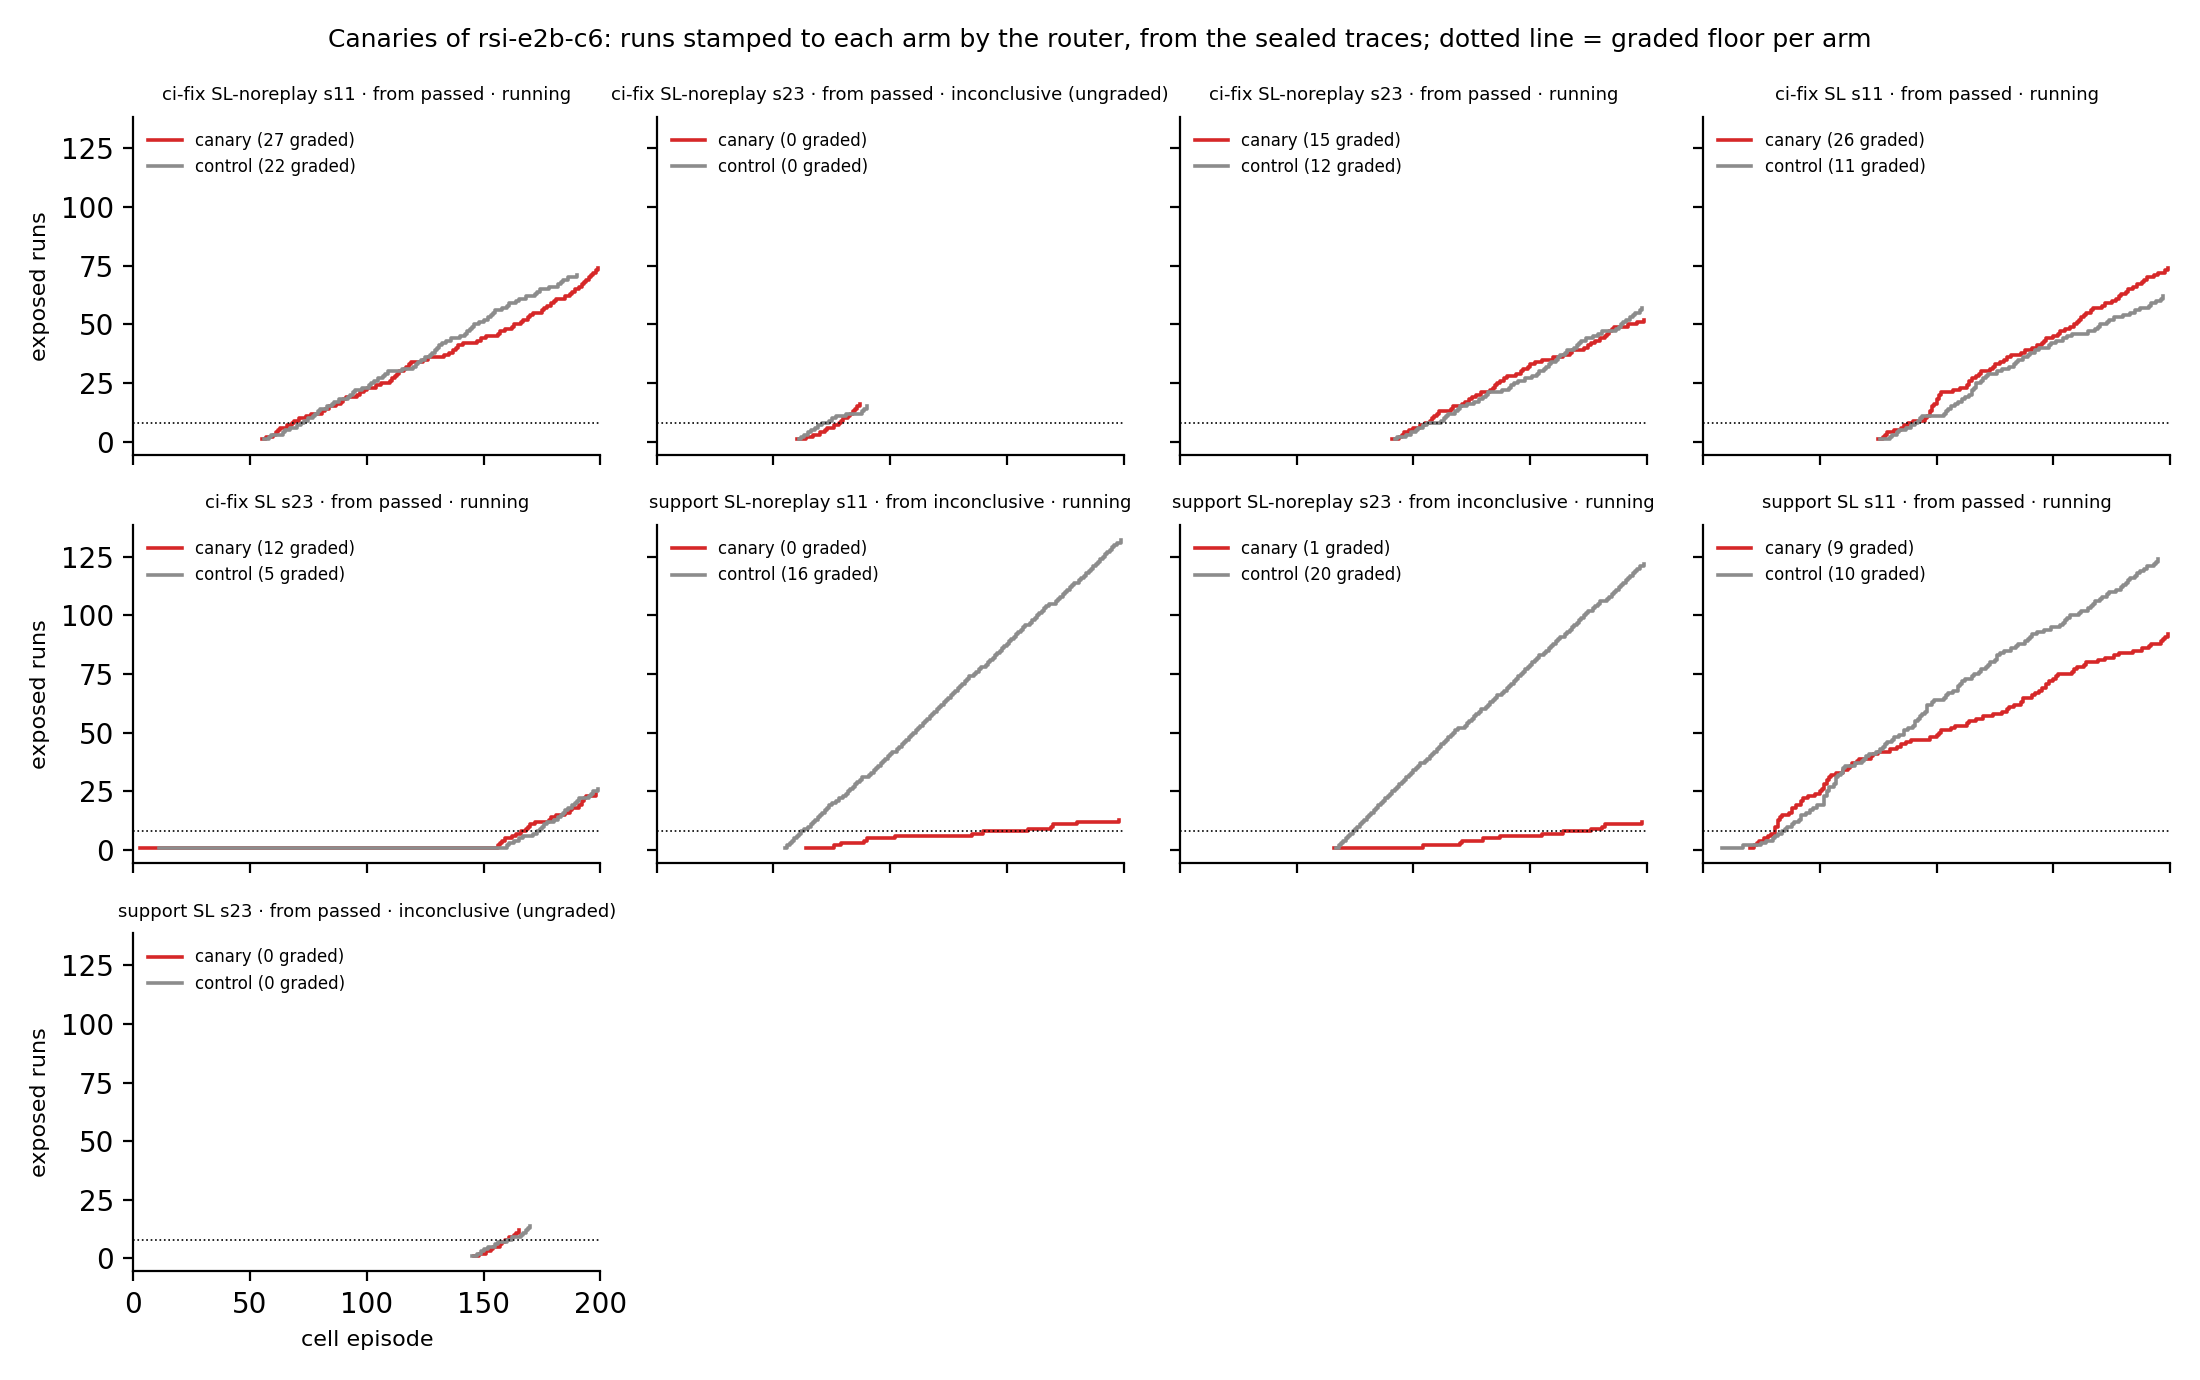
\includegraphics[width=\textwidth]{figures/fig_canary.png}
\caption{The nine canaries of \code{rsi-e2b-c6} (fleet 10, 200 episodes, change at 50), each
panel one fix: runs the router stamped to the canary arm (red) and the control arm (grey) by cell
episode, from the sealed traces; dotted line = the graded floor of 8 per arm; the legend gives
how many stamped runs the canary could grade. Canaries started from an inconclusive Tier~1
route 10\,\% of traffic to the fix, the rest 50\,\%. Four reached the floor on both arms; none
decided --- three because the failure no longer recurred in control, one because 9 and 10 graded
runs leave the non-inferiority bound at 14 points against a margin of 10.}
\label{fig:canary}
\end{figure}

\subsection{SenseLab by engine cut}

\begin{table}[H]
\centering\scriptsize\setlength{\tabcolsep}{3pt}
\resizebox{\linewidth}{!}{\begin{tabular}{lrrrrrrr}
\toprule
\textbf{engine cut} & \textbf{moved half} & \textbf{kept half} & \textbf{unchanged} & \textbf{escalated} & \textbf{fixes proposed} & \textbf{Tier 2 passed} & \textbf{shipped} \\
\midrule
pre-seam4 (`rsi-c1-rsi`) & 36 \% (27/75) & 65 \% (42/65) & 96 \% (134/139) & 6 \% (22/399) & 9 & 2 & 0 \\
post-seam5 (`rsi-c2`) & 47 \% (35/75) & 60 \% (39/65) & 99 \% (138/140) & 6 \% (24/400) & 16 & 6 & 0 \\
post-seam5b (`rsi-c3`) & 43 \% (32/75) & 60 \% (39/65) & 99 \% (138/140) & 8 \% (30/400) & 24 & 15 & 0 \\
post-clean-success (`rsi-c5`) & 34 \% (25/74) & 63 \% (41/65) & 96 \% (132/137) & 8 \% (33/396) & 16 & 3 & 0 \\
post-canary-ni (`rsi-c6`) & 33 \% (25/75) & 63 \% (41/65) & 96 \% (134/140) & 8 \% (32/400) & 13 & 4 & 0 \\
\bottomrule
\end{tabular}}
\caption{SenseLab on successive cuts of the engine, same protocol and seeds. Fix counts are over the four SenseLab cells of each run. \code{pre-seam4}: amfs-internal \#787/\#788; \code{post-seam5}: \#793, \#794; \code{post-seam5b}: \#795, \#796; \code{post-clean-success}: \#797, \#798; \code{post-canary-ni}: \#799 (\S\ref{sec:findings}).}
\label{tab:cuts}
\end{table}



\begin{figure}[H]
\centering
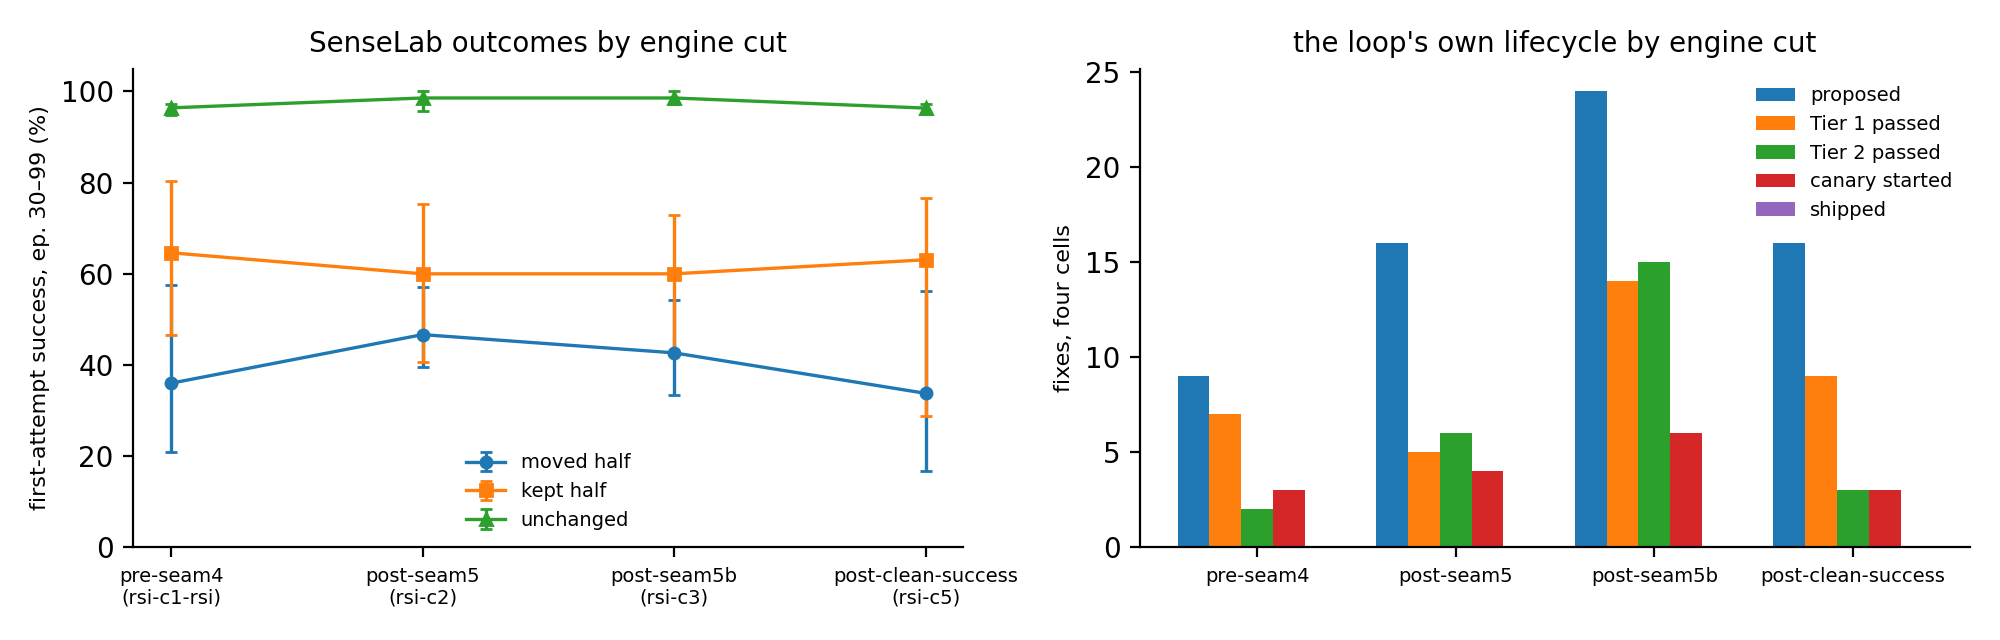
\includegraphics[width=\textwidth]{figures/fig_cuts.png}
\caption{SenseLab on successive cuts of the engine, same protocol and seeds. Left: outcome
endpoints, which move within their intervals. Right: the loop's own lifecycle counts over the
four cells --- what it proposed, what passed Tier~1 and Tier~2, how many canaries started and
what shipped (nothing, on every cut: no canary decided inside a 100-episode cell).}
\label{fig:cuts}
\end{figure}

Table~\ref{tab:cuts} is the same protocol on successive cuts of the engine and is the trace of
\S\ref{sec:findings} in numbers: the loop went from 9 proposals and 2 Tier~2 passes on the first
cut to 24 and 15 on the third as its evidence path was repaired, then to 16 and 3, and 13 and 4,
as the proof learned to reject a recovered success --- while the outcome endpoints moved within
noise throughout. The cut under test now is the first on which the proof set can see the
conditional and the drafter is shown the runs the old rule still serves.

\subsection{Cost}
\label{sec:cost}

\begin{table}[H]
\centering\scriptsize\setlength{\tabcolsep}{3pt}
\resizebox{\linewidth}{!}{\begin{tabular}{lrrrrrrrrrr}
\toprule
\textbf{system} & \textbf{tokens/ep} & \textbf{agent \$/ep} & \textbf{arm \$/ep} & \textbf{judges \$/ep} & \textbf{replays \$/ep} & \textbf{drafts/100 ep} & \textbf{drafts \$/ep (est.)} & \textbf{total \$/ep} & \textbf{memory s/ep} & \textbf{wall s/ep} \\
\midrule
Frontier alone & 1,287 & 0.011 & 0.000 & 0.000 & 0.000 & 0.0 & 0.000 & 0.011 & 0.0 & 5 \\
Context window & 24,322 & 0.070 & 0.000 & 0.000 & 0.000 & 0.0 & 0.000 & 0.070 & 0.0 & 4 \\
pgvector & 4,475 & 0.027 & 0.000 & 0.000 & 0.000 & 0.0 & 0.000 & 0.027 & 0.0 & 9 \\
pgvector + rerank & 3,953 & 0.025 & 0.003 & 0.000 & 0.000 & 0.0 & 0.000 & 0.028 & 0.0 & 10 \\
pgvector + outcomes (DIY) & 5,406 & 0.029 & 0.005 & 0.000 & 0.000 & 0.0 & 0.000 & 0.035 & 0.0 & 9 \\
SenseLab & 6,629 & 0.033 & 0.000 & 0.004 & 0.004 & 3.0 & 0.004 & 0.046 & 14.8 & 25 \\
SenseLab $-$ canary & 6,581 & 0.033 & 0.000 & 0.005 & 0.007 & 3.5 & 0.005 & 0.049 & 14.1 & 24 \\
SenseLab $-$ repair loop & 6,537 & 0.032 & 0.000 & 0.000 & 0.000 & 3.8 & 0.005 & 0.037 & 10.5 & 20 \\
\bottomrule
\end{tabular}}
\caption{Cost and latency per episode, by where the call is charged. \emph{agent \$}: the agent's own calls; \emph{arm \$}: reflection or consolidation the arm ran per episode; \emph{judges \$} and \emph{replays \$}: the loop's judge verdicts and the Tier~2 replays the harness re-ran on the fix branch, exact from the run records; \emph{drafts}: fixes the repair agent drafted per 100 episodes, priced at the account ledger's remainder per draft (repair agent, Tier~1 stand-in replay, lever classification, discovery --- not persisted per fix, so an estimate; \S\ref{sec:cost}). \emph{total} sums the five. \emph{memory s}: time in memory calls against the production API.}
\label{tab:cost}
\end{table}



\begin{figure}[H]
\centering
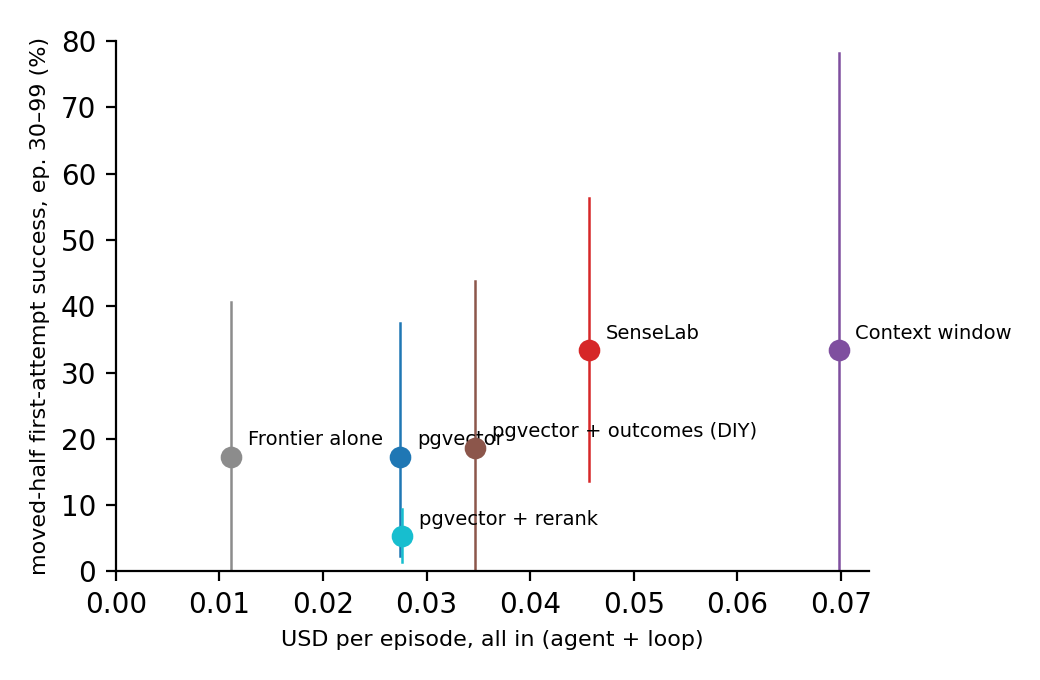
\includegraphics[width=0.62\textwidth]{figures/fig_cost.png}
\caption{Recovery on the moved half against all-in cost per episode, the loop's own spend
included (Table~\ref{tab:cost}); vertical bars are the cell-level bootstrap intervals.}
\label{fig:cost}
\end{figure}

Every call is charged to the system that caused it, wherever it ran. The agent's own calls are
in the episode records. The loop's platform-side calls are on the benchmark account's evaluation
ledger, which settles every judge verdict, repair-agent step, stand-in replay, lever
classification and discovery call as it happens; judge verdicts also carry their own cost, and
every verdict and every Tier~2 replay of a cell is in the run record, so those two columns are
exact per cell. The repair agent's spend is not persisted per fix. It is recovered as the
ledger's remainder --- what the account spent minus what its judges cost, over every fix the
agent drafted on the account (USD~0.135 per draft at the time of writing, from USD~77.6 spent, 39.1
of it judges, over 285 drafts) --- and applied per cell as drafts~$\times$ that rate; the column
says \emph{est.} because it is one. Runs launched from the day the ledger was first snapshotted
carry a reading at run start, after every cell and at run end, so the confirmatory runs report
the ledger difference directly and this estimate is checked against it.

On these seeds SenseLab costs USD~0.046 per episode all in: 4.2$\times$ the frontier model alone
(0.011), 1.3--1.7$\times$ the pgvector memories (0.027--0.035), and 0.66$\times$ the context window
(0.070). A quarter of it is the loop (judges 0.004, Tier~2 replays 0.004, drafts 0.004 per
episode); the rest is the agent reading a longer briefing than a top-5 retrieval. Holding the
loop at review still drafts (3.8 proposals per 100 episodes, 0.037 per episode): the drafting
is what a person would read. Memory time (15\,s per episode against the production API, under
the harness's rate pacing) is the price of reading the evidence record rather than a vector
index.

\subsection{Two probes on the earlier change set}

\paragraph{When the team grows.} On the unconditional change (set A, change at 20), with a fleet
of six agents sharing one store: in the \emph{pioneer} protocol one agent works alone for 60
episodes and five join; in the \emph{newcomer} protocol five work and a sixth joins at 60. A
joiner on SenseLab takes the post-change action on its first exposure to a changed class in
36/36 (pioneer) and 10/10 (newcomer) cases with zero stale picks; a joiner on pgvector + rerank
does so in 31\,\% and 40\,\% with 17\,\% and 0\,\% stale picks and 16--20\,\% escalations. The
inheritance is the outcome record, not the notes: the same notes are in both stores.

\begin{table}[H]
\centering\scriptsize\setlength{\tabcolsep}{3pt}
\resizebox{\linewidth}{!}{\begin{tabular}{lrrrrrrr}
\toprule
\textbf{arm} & \textbf{veterans ep50-59 1st} & \textbf{veterans changed post 1st} & \textbf{joiner 1st-exp all} & \textbf{1st-exp changed} & \textbf{1st-exp unchanged} & \textbf{stale-pick (changed 1st-exp)} & \textbf{escalated} \\
\midrule
pgvector + rerank & 0.75 & 0.28 & 0.68 [0.52,0.83] (n=90) & 0.31 [0.15,0.50] (n=36) & 0.93 [0.78,1.00] (n=54) & 0.17 & 0.20 \\
SenseLab & 1.00 & 0.76 & 1.00 [1.00,1.00] (n=90) & 1.00 [1.00,1.00] (n=36) & 1.00 [1.00,1.00] (n=54) & 0.00 & 0.00 \\
\bottomrule
\end{tabular}}
\caption{When the team grows (set A, change at 20, fleet of six sharing one store; \emph{pioneer}: one agent works alone to episode 60, five join). First-attempt success of the joiners on their first exposure to each class after joining, with the veterans' rate before they joined; \emph{stale-pick}: the joiner applied the pre-change action.}
\label{tab:teamgrows}
\end{table}


\paragraph{A student trained on the record (E7 at rung 0).} Two Managed Models
(\code{senselab-s1}) were trained on the dev-seed \code{support} traces of SenseLab and of the
ablation without the repair loop (200 traces each), and evaluated on held-out seeds 101/113/127
(1,500 episodes). Alone, neither student takes the new action first (9\,\% and 0\,\% on the moved
half); with SenseLab's outcome loop as its memory each does (33\,\% and 30\,\%), at 1/23 of the
frontier model's cost per episode --- and beats GPT-5.5 with the same memory (22\,\%) on the moved
half at this rung, which is the contamination the evaluation ladder exists to expose: rung 0 uses
the training classes. The SenseLab-trained student against the ablation-trained one is
$-7/0/+18$ points across the three seeds --- ``small and reported as such'' is the preregistered
sentence. Nothing is claimed from rung 0; rungs 1--3, on classes and wordings the students never
saw, need eval-only content that is registered but not yet written.

\section{Confirmatory results}
\label{sec:confirmatory}

The seeds 37, 41, 59 and 73 run once, on both agent models, after the analysis code is tagged
\code{analysis-freeze-rsi}; every table in this section is filled by that frozen code from the
confirmatory read and nothing in it is known when the freeze is made. The endpoints, the paired
test (exact two-sided sign-flip over the sixteen cells, Holm across the five systems on the
primary endpoint, Holm within each secondary endpoint) and the tables are those of
amendments~(w) and~(x); the development-seed tables of \S\ref{sec:results} are not re-read.
The prose of this section is written after the read and states, for each preregistered
prediction, whether it was met.

\paragraph{Primary endpoint: the moved half.}
\textcolor{red}{[pending: the confirmatory seeds have not run; this table is filled from \code{results/rsi-report-confirmatory} --- ``1. After the rule changes conditionally''.]}
\textcolor{red}{[pending: the confirmatory seeds have not run; this table is filled from \code{results/rsi-report-confirmatory} --- ``1b. Paired cell deltas, moved half''.]}

\paragraph{Secondary endpoints: collateral damage.}
\textcolor{red}{[pending: the confirmatory seeds have not run; this table is filled from \code{results/rsi-report-confirmatory} --- ``1b-kept. Secondary endpoint, paired: kept half''.]}
\textcolor{red}{[pending: the confirmatory seeds have not run; this table is filled from \code{results/rsi-report-confirmatory} --- ``1b-unchanged. Secondary endpoint, paired: unchanged classes''.]}

\paragraph{By family and by model.}
\textcolor{red}{[pending: the confirmatory seeds have not run; this table is filled from \code{results/rsi-report-confirmatory} --- ``1c. By family''.]}
\textcolor{red}{[pending: the confirmatory seeds have not run; this table is filled from \code{results/rsi-report-confirmatory} --- ``1d. By model''.]}

\paragraph{Attribution and the loop's lifecycle.}
\textcolor{red}{[pending: the confirmatory seeds have not run; this table is filled from \code{results/rsi-report-confirmatory} --- ``3. Attribution''.]}
\textcolor{red}{[pending: the confirmatory seeds have not run; this table is filled from \code{results/rsi-report-confirmatory} --- ``4. Fix lifecycle''.]}

\paragraph{Where canaries can decide: fleet 10, 200 episodes.} The E2b protocol on the four
confirmatory seeds (SenseLab, $-$canary, $-$replay; 4,800 episodes per seed) is read with the
canary readout of amendment~(v): P12 (canaries reach the graded floor on both arms), P13
(canaries decide), P14 (no pass harms the kept class by more than the margin, joined to the
sealed traces' arm stamps) and P11(a$'$) (drafts state their condition, two blind coders).
\textcolor{red}{[pending: the fleet-10 confirmatory cells have not run.]}

\paragraph{Cost.}
\textcolor{red}{[pending: the confirmatory seeds have not run; this table is filled from \code{results/rsi-report-confirmatory} --- ``5. Cost and latency''.]}

\section{What the loop taught us about itself}
\label{sec:findings}

The preregistration promised to report every prediction. Table~\ref{tab:ledger} is that report,
and the findings below are the record of what a benchmark that knows the true rule found in a
shipped self-improvement loop --- nine defects and two properties of the problem --- none of
which a retrieval benchmark could have seen. All nine were fixed in production between runs, with
their deploy cuts recorded, and all nine re-measured on the same protocol in the fleet-1 run the
headline tables report; the ninth was found in the fleet-10 run, and its fleet-10 re-measurement
is the run this version reports as open. We think this section is the paper's main contribution; the loop's evidence path
is where such systems fail, and none of these failures is specific to ours.

\begin{enumerate}[leftmargin=1.6em, itemsep=0.35em]
\item \textbf{The loop was never reached.} (Pilots 5b--5g.) Incidents open at three failing
verdicts on one behaviour cluster; a fresh agent's judges had graded nothing, so no incident
opened and no fix was proposed in 60 episodes. The regime-shift producer --- an entry validated
$\geq 3$ times that now fails --- is the producer a memory can drive without judges, and it is what
every result here rests on.
\item \textbf{Sealing stalled under load.} A lock on the seal path held sessions open under the
grid's concurrency; fixed (\#780/\#781) before any reported run.
\item \textbf{A first-exposure failure is not a regime shift.} (Amendment (k), pilot 5k; P1
falsified 3/3.) The shift producer fired on entries that had been \emph{read}, not validated,
so the first failure of a never-tested entry opened a canary that could grade nothing --- the
canary compares recurrence of a failure the control arm had never had. The guard now requires
validation in the situation.
\item \textbf{On an unconditional change, demotion recovers almost everything.} (Amendment (l);
P4.) A scripted maintainer writing the true rule five episodes after the change beat outcome
learning alone by 2.5 (\code{support}) and 4.2 (\code{ci-fix}) points on 60 episodes of set A.
That is the ceiling a repair loop can reach on such a change, and it is small. Change set C
was written so that demotion has no signal: the entry is still right on the kept half.
\item \textbf{A regime fix had nothing to be proved against.} (Seam 4, \#793; P6 met on the
ablation.) Case sets were built from judge verdicts; a fix drafted from a shift had none, so
Tier~2 could not be asked and \code{auto\_after\_replay} had nothing to ship on. The manifest's
runs now seed the case set, and a judge-less case is graded on the replay's outcome.
\item \textbf{The agent spells one situation ten ways.} (Seam 5, \#794; P7 recall 0.71, purity
0.92 against 0.80/0.90 predicted; seam 5b, \#796, P7$'$ falsified: 0.40/0.67.) A canary scoped to
a situation graded 2 of 15 in-situation runs because the agent labelled the same situation
\code{csv export timeout}, \code{data export error}, \code{large export failing}. A server-side
canonical resolves labels by stemmed tokens; the embedding second stage added for recall
\emph{lowered} it and merged \code{ci-fix} classes (\code{format check failure}
$\sim$ \code{audit check failure} at 0.79). It is left on by decision, with its cost stated.
\item \textbf{A running canary swallowed every later fix's replays.} (Seam 7, \#795; P8 met.)
The router bucketed a Tier~2 replay session like any other; a replay for fix $B$ sealed during
$A$'s canary was stamped onto $A$'s branch, counted in $A$'s arm, and reported \code{missing} to
$B$. Replays are now re-stamped onto their own branch and excluded from every canary tally.
\item \textbf{The loop drafted fixes from its own tests.} (Seam 8, \#797; P10 pending.) A Tier~2
replay that failed on a fix branch read to the regime pass as the entry failing on \code{main}:
13 of 40 fixes on the \code{post-seam5b} cut were drafted from a replay, in chains --- a fix from
the replay of a fix from a replay --- and one replay's spelling became a canonical that four
served runs then joined. Replays are no longer traffic at the seal: no judge, no identity, no
shift. (The first cut of this rule also excluded the labelled copy of a served inference, which
is traffic; an automated reviewer caught it before merge.)
\item \textbf{The proof graded the wrong signal.} (Amendment (s), \#797; P9(b) falsified 20/24,
P11 pending.) See \S\ref{sec:results}: an outcome-graded case passed a recovered success, so an
unconditional flip passed a proof set built to catch it. A case now passes only on a clean success
--- no recorded failed attempt --- and the change is dated by the case, not the deploy, so earlier
case sets keep their semantics.
\item \textbf{Who grades the proof.} (Found while this version was being written; fix pending
approval.) The clean-success rule of finding 9 applies to a case no judge graded. In this
benchmark 174 of 175 proof cases carry a judge --- the benchmark's own frozen rubric, which the
continuous-judging tier had already run on the evidence trace --- and that rubric says, by
design, that ``a run that failed one or more attempts before succeeding is a PASS''. The proof
tier therefore inherits the coarse signal through the judge as well as through the outcome, and
finding 9's fix reaches one case in 175 here. The size of the leak is measurable: of the 555 case
replays run since the \code{post-seam5b} cut, 479 passed, and 116 of those passes (24\,\%) carry
a recorded failed attempt --- a recovered success the proof counted as clean. The engine-side correction is to carry the
clean-success requirement on every case built for a regime fix, whatever grades it, and enforce
it after the verdict. It shipped as the \code{post-clean-success} cut; P11 is read on the run
on that cut (\S\ref{sec:pending}), and Table~\ref{tab:cuts} carries it as a row.
\item \textbf{The canary grades by canonical situation, and the agent's declarations fragment.}
(Found in the fleet-10, 200-episode run of \S\ref{sec:posthoc}; fixed in \#799 and re-measured
on both protocols.) A canary counts
exposure --- runs that read the fix's entry --- but grades only runs whose canonical situation
equals the fix's. The agent declares its situation per run in its own words, often carrying the
very condition the change turns on (``pip audit requests pin with legacy sdk'', ``pip audit
requirements plus nonclient code''); situation identity folds one agent's 56 declarations to 10
canonicals, the pip-audit ones to ``pip audit failure'' --- while the fixes carry ``pip audit
pinned change'' and two more, assigned when each was proposed. So 0--8 of 16--30 exposed runs per
arm are graded, three canaries end ``none declared it'', and no canary decides in 200 episodes
with ten agents; the one whose declarations were stable reached 25/30 graded, found recurrence of
12\,\% against 17\,\% --- no significant difference --- and timed out, because the rule waits for
a significant \emph{improvement}. This, not the horizon, is why no canary has decided in any run.
Corrected after approval (amendment~(v), PR~\#799, cut \emph{post-canary-ni}): the canary grades
runs in the fix's situation \emph{or} that read an entry the fix is about, and its primary is
non-inferiority --- a one-sided 95\,\% Newcombe bound on canary$-$control recurrence under 10
points, with the failure live in control --- because the canary is the harm gate on a change the
replay tiers already proved. Canonical merging was not done: it changes situation identity for
every customer with the opposite failure mode, and the canary no longer depends on it.
Pre-registered on the rerun: P12 (canaries reach the floor), P13 (canaries decide), P14 (no pass
harms the kept class) and P11(a$'$) (drafts state their condition; the regime draft now sees the
situation's passing runs). Re-measured (\S\ref{sec:posthoc}): graded runs rose from 0--27\,\% of
exposure to 12--55\,\%, four of nine canaries reached the floor, and none decided --- three
because the failure had stopped recurring in control by the time the canary could measure it.
The grading defect is closed; what the rerun shows is that the canary's evidence arrives after
the fleet has recovered on its own, which is a property of the problem at this horizon rather
than a defect.
\end{enumerate}

\paragraph{The canary inside a cell (see also \S\ref{sec:posthoc}).} Separately from the defects, no canary reached a decision
inside any 100-episode cell (K1--K4 in the readouts): a situated canary grades only in-situation
runs, and at \code{pct}=50 with a floor of 8 per arm it needs 16 in-situation graded sessions
after it starts, which a cell with 4--10 post-change exposures of one class cannot supply. This
is a property of the protocol, not a defect; the flagship long-horizon experiment (200 episodes,
fleet 10) is sized for it, and Table~\ref{tab:attribution}'s ``$-$ canary'' row is the reading of
what ships when the gate is the replay alone.

\begin{table}[H]
\centering\scriptsize
\begin{tabular}{llp{6.2cm}l}
\toprule
\textbf{P} & \textbf{Where} & \textbf{Prediction (dev seeds, set C unless stated)} & \textbf{Verdict} \\
\midrule
P1 & (k) 5k & a shift-drafted fix is graded on runs that read the entry & falsified 3/3 \\
P2 & (l) c1 & $-$ canary ships a regime fix in every cell; recurrence falls & not met (1/4) \\
P3 & (l) c1 & SenseLab's canary reaches a decision in-cell & not met (K1--K4) \\
P4 & (l) 5A & maintainer oracle within 3 pts of outcome learning, set A & +2.5 / +4.2 \\
P5 & (l) & judges-only recovers $\geq 0.7$ of oracle recovery & pending \\
P6 & (o) c2 & every Tier~1-passed regime fix gets a Tier~2 verdict & met (ablation); falsified by seam 7 (SenseLab) \\
P7 & (o) c2 & situation recall $\geq 0.80$, purity $\geq 0.90$ & 0.71 / 0.92 \\
P7$'$ & (r) c3 & embedding stage: recall $\geq 0.80$, purity $\geq 0.90$ & falsified 0.40 / 0.67 \\
P8 & (q) c3 & replays during a canary are re-stamped and graded & met (26/26) \\
P9(a,c) & (q) c3 & proof set of 3--6 cases; kept-case failures occur & met \\
P9(b) & (q) c3 & $\leq 25\,\%$ of proof-passing regime fixes non-conditional & falsified 83\,\% \\
P10 & (s) c5 & no fix drafted from a replay; no alias from a replay & met (0 of 47 manifest runs; 134 replays present) \\
P11 & (t) c5 & non-conditional share $< 50\,\%$; a \code{ci-fix} kept-case failure; ships fall & (a) falsified 4/4; (b) met, 3; (c) met, 11 $\to$ 2 \\
P12 & (v) c6 & $\geq 1$ in 2 canaries reach the graded floor on both arms; graded/exposed $\geq 0.8$ & not met: 4 of 9; graded/exposed 0.12--0.55 (from 0--0.27) \\
P13 & (v) c6 & $\geq 1$ in 3 canaries decide & falsified: 0 of 9 (7 from Tier~1 pass, 2 from inconclusive); 3 of 4 at the floor had 0 recurrence in both arms \\
P14 & (v) c6 & no pass harms the kept class by $> 10$ pp (trace-joined) & undefined: no verdict \\
P11(a$'$) & (v) c6 & $\geq 50\,\%$ of kept-case regime drafts state a condition (two blind coders); kept-case rejections $< 5$ of 23 & coding pending (37 items over \code{rsi-c6}, \code{rsi-e2b-c6}); rejections 4 of 17 and 11 of 39 --- the count fell, the share did not \\
\bottomrule
\end{tabular}
\caption{The predictions ledger. Every preregistered prediction on the engine so far, with the
amendment that made it, the run that tested it and its verdict. Pending rows are being tested on
the run this version reports as open.}
\label{tab:ledger}
\end{table}

\section{Pending, and what we expect}
\label{sec:pending}

The headline tables are the run on the current cut, \code{post-canary-ni} (findings 8--11
live; \code{rsi-c6}). The two predictions preregistered on the cut before it were read on that
cut's run (\code{rsi-c5}) and stand as follows. \textbf{P10} (no fix has a manifest run that is a replay; no situation alias is created
by a replay) is met: of the 47 runs cited by the 33 fix manifests drafted since the cut, none
carries a replay tag, while 134 of the 928 sessions sealed in the same window were replays; and
the seal hook sets a replay aside before situation identity runs, so no alias can come from one.
\textbf{P11} had three clauses. (a) The share of proof-passing regime fixes that do not encode the
conditional falls below 50\,\% from 83\,\% --- \emph{falsified}: 4 of 4. (b) At least one regime
fix fails Tier~2 on a kept case on \code{ci-fix} --- met, 3. (c) The number of ships falls ---
met, 11 to 2 in the ablation, with SenseLab's Tier~2 passes falling from 15 to 3. The falsification
of (a) is informative in the way the preregistration anticipated: the proof now removes 19 of 23
regime fixes, and the four survivors are wholesale flips whose kept-half replays passed because
the replaying agent did not follow the entry. Where the conditional is lost is therefore now
located --- in the repair agent's draft, not in the proof --- and the two remaining instruments are
the live canary, which grades what agents actually do with the entry, and the followed-memory
criterion, which separates a wrong rule from a wrong rule that was followed. The drafting change
that followed (amendment (v): state the condition that separates the failing runs from the
passing ones, with the passing runs in hand) is live on the current cut, and P11(a$'$) reads it: of
the regime fixes whose proof set holds a kept case, at least half state a condition, judged by two
coders blind to arm and verdict. On \code{rsi-c6} that population is 12 fixes; the sheet is
drawn and the coding is pending. Our own reading of the two proof passers (\S\ref{sec:results})
is not that count. The second clause of P11(a$'$) --- kept-case proof rejections fall below 5 of
23 --- reads 4 of 17 on this cut and 11 of 39 on the fleet-10 rerun: fewer in number where the
run is the same size, the same or a higher share.

\textbf{P12--P14} are read on the fleet-10 rerun (\code{rsi-e2b-c6}, \S\ref{sec:posthoc}).
P12: 4 of 9 canaries reached the graded floor on both arms (not met at $\geq 1$ in 2; not
falsified), and no canary graded 80\,\% of the runs that read its entry (0.12--0.55; before the
correction 0--0.27). P13: 0 of 9 decided --- \emph{falsified}. P14: undefined, no verdict. The
falsification of P13 is the informative one. Three of the four canaries at the floor had zero
recurrence in both arms: the harm gate had nothing to gate because the fleet had stopped making
the mistake before the gate could measure it. Whether a fix for a failure that no longer recurs
should ship anyway --- as a written condition for the next agent, rather than a live correction
--- is an engine question we put to the owner and do not answer here; the confirmatory fleet-10
cells are read with P12--P14 as pre-specified. Why a canary grades only a third to a half of the
runs that read its entry, after the correction that was meant to close that gap, is not
diagnosed in this version.

\paragraph{The confirmatory scope, reduced before it ran.} Amendment (w), declared before any
confirmatory-seed cell and before the analysis freeze, reduces the confirmatory grid to what the
paper's claims rest on: seeds 37/41/59/73 on the two set-C families (\code{support},
\code{ci-fix}), both agent models (GPT-5.5 and Claude Opus~5), fleet~1 on the C protocol with
every system in Table~\ref{tab:headline} and both ablations, and fleet~10 on the E2b protocol
(200 episodes, change at 50) with SenseLab and its two gate ablations --- 22,400 episodes on the
\code{post-canary-ni} cut. The loop has not been run on the remaining eight families: they appear
only in the level-0 comparison of the earlier ten-family grid (SenseLab with the loop held,
against the same baselines, change sets A and B, development seeds), cited as such; their
held-out set~C is not authored, and the held-out-family design of amendment (l) lapses with it. The paired test is the exact sign-flip
test over cells with Holm across systems (amendment (x)); the mixed-effects learning-curve model
named in the preregistration is not run, for the reasons given there. What is not run at all and
is reported as not run: verdict sources (E3), the public track (E4), the A/A, adversarial,
reward-hacking and manifest-calibration probes, and the Managed Model rungs above L0 (E7). Each
is a claim this paper does not make.

\section{Related work}

\paragraph{Self-improvement.} Self-Refine~\cite{selfrefine} and STaR~\cite{star} improve a model's
outputs or weights from its own feedback within a task or a training run. The Gödel machine
lineage~\cite{godel,dgm} and AlphaEvolve~\cite{alphaevolve} modify the improver itself, gated by a
proof or a benchmark score, in a sandbox. The engine here is the deployed case: the object it
modifies is what every live agent acts on, the gate is live traffic rather than a held-out
score, and the discipline --- manifest, tiers of proof, staged exposure, reversibility, an
audit trail --- is the contribution rather than the search. The ``fixed budget, held-out,
sustained, generalising'' conditions that the preregistration adopts for any claim of
self-improvement (E5) are the four conditions Weco proposes for the ``net positive'' rung of its
ladder of recursive self-improvement~\cite{weco-ladder} and reports meeting with
AIDE$^2$~\cite{weco-aide2}: a fair human baseline, a sustained multi-step trend, generalisation
beyond the optimised measurement, and a fixed budget. (The ladder's rungs number the strength of
the claim; the levels of this paper number the stages of one loop. The two numberings are
unrelated.) E5 has not run (\S\ref{sec:pending}); no rung is claimed.

\paragraph{Release engineering.} Canary release and controlled online experiments
\cite{kohavi} are the discipline the loop borrows for level~1; A/A tests and look-schedule
inflation are the standard hazards, and the preregistration's A/A probe measures the empirical
false-pass rate of the canary's test under the schedule the harness uses.

\paragraph{Benchmarks.} $\tau$-bench and $\tau^2$-bench~\cite{taubench,tau2bench} evaluate
tool-using agents against a policy that stays fixed across tasks; our public track (E4) amends the
policy between passes to ask this paper's question on a public task set. Continual-learning
benchmarks for language models measure forgetting in weights; the object here is what a deployed
agent acts on, and the failure mode is remembering.

\paragraph{Agent memory, as substrate and as baseline.} Reflexion~\cite{reflexion} and
Voyager~\cite{voyager} write verbal reflections and skills back for later episodes; Generative
Agents~\cite{genagents} and MemGPT~\cite{memgpt} manage a store with retrieval and summarisation;
Mem0~\cite{mem0} and Zep~\cite{zep} are production memory layers evaluated on conversational
recall (LoCoMo, LongMemEval~\cite{longmemeval}). All are evaluated on retrieving what was stored;
none tests, gates or reverts a change to the store, and none is measured on a change of the world
after storage. They are the substrate a self-improving engine operates on and the baselines it is
measured against here; our earlier report~\cite{senselab-cl} measured level~0 against these
designs under a regime change.

\section{Threats to validity}

\begin{itemize}[leftmargin=1.4em, itemsep=0.25em]
\item \textbf{Development seeds.} Every number is from two seeds on two families, chosen for
development. The confirmatory seeds run once after the freeze; nothing here is a confirmed
difference, and the intervals say so.
\item \textbf{One model, one effort level.} GPT-5.5 at low effort. Claude Opus 5 has not run on
set C on the development seeds; it is half of the confirmatory grid (amendment (w)), where every
cell is model-aware.
\item \textbf{The benchmark's outcome is coarse.} The harness reports \code{success} for an episode
solved within three attempts; that is what the customer reports, and it hid finding 9 from the
proof set for two runs. The clean-success rule reads the attempts the agent already records; a
customer whose agent never records attempts sees no change and gets no protection.
\item \textbf{The engine changed between runs.} Nine defects were fixed in production during the
study (amfs-internal \#780--\#799). Every result carries its cut; latency claims are within one cut
only; and the changes are to the loop's evidence path, not to any threshold constant, which the
preregistration forbids. The one gate rule that changed --- the canary's primary, from
superiority to non-inferiority (finding 11) --- was preregistered with its falsifier before the
run that tests it.
\item \textbf{The loop's drafting cost is an estimate.} Judge verdicts and Tier~2 replays are
charged exactly per cell; the repair agent's spend is the account ledger's remainder spread over
every draft on the account (\S\ref{sec:cost}), so a cell that drafted long fixes is under-charged
and one that drafted short ones over-charged. The confirmatory runs snapshot the ledger per cell
and report the difference directly.
\item \textbf{Hand-coding.} The ``non-conditional'' share (P9(b), P11) is a reading of the shipped
text against the known change by one coder; the confirmatory run will use two, blind to arm.
\item \textbf{The harness routes the canary.} The production router runs in the MCP gateway; the
harness applies the same hash itself (parity-tested in CI) because it talks to the HTTP API.
\item \textbf{The context window is a strong baseline where it fits.} On \code{ci-fix} the whole
cell fits in 24k tokens and the window sees the change; it is the right comparison for short
horizons and the wrong one for the 200-episode fleet, where it cannot fit.
\item \textbf{We built the system.} The preregistration, the amendments with their falsifiers,
the cut records and the ledger exist so that a reader can check what was predicted before each
run rather than take our reading of it.
\end{itemize}

\appendix
\section{Reproducibility}

\paragraph{Runs.} Harness arm names, cell ids and command lines: baselines
\code{rsi-c1-tier1} (\code{none}, \code{pgvector+rerank}, \code{senselab}),
\code{rsi-c1-baselines} (\code{pgvector}, \code{pgvector-diy+outcomes}),
\code{rsi-c1-baselines-cw} (\code{raw-traces}); SenseLab \code{rsi-c1-rsi}, \code{rsi-c2},
\code{rsi-c3}, \code{rsi-c5}, \code{rsi-c6} (\code{senselab-rsi}, \code{senselab-rsi-nocanary}); fleet~10
\code{rsi-e2b-c5}, \code{rsi-e2b-c6} (plus \code{senselab-rsi-noreplay}, 200 episodes, change at 50,
\code{-rep}); confirmatory \code{rsi-conf-f1-s<seed>} and \code{rsi-conf-e2b-s<seed>} from
\code{confirm\_rsi.sh}. Cell id
\code{<family>|<arm>|gpt-5.5|s<seed>|} \code{e100-d300-n0.0-f0-a1-c30-x0.5-oid-vC}. Command:
\begin{quote}\scriptsize\ttfamily\raggedright python -m continual\_learning.runner --run <run> --scenarios support ci-fix --arms <arms> --models gpt-5.5 --seeds 11 23 --fleet 1 --episodes 100 --change-at 30 --change-focus 0.5 --change-variant C --opaque-ids --workers 2\end{quote}
with \code{CL\_RSI\_TIER2=1} and a Tier~2 replay receiver reachable from the service.

\paragraph{Engine cuts.} \code{pre-seam4}: amfs-internal \#787/\#788. \code{post-seam5}: \#793
(07:00:22Z), \#794 (08:27:24Z, 2026-09-27). \code{post-seam5b}: \#795 (12:50:24Z), \#796
(13:39:13Z). \code{post-seam8}: \#797 (09:14:17Z, 2026-09-28). \code{post-clean-success}: \#798.
\code{post-canary-ni}: \#799 (11:35:32Z, 2026-09-29). Each cut's Cloud Run revision is in
\code{HYPOTHESIS\_RSI.md}.

\paragraph{Analysis.} \code{python -m benchmarks.continual\_learning.analysis.rsi --paper} writes
\code{results/rsi-report/REPORT.md} and \code{report.json} for the development seeds;
\code{--seeds 37 41 59 73 --models gpt-5.5 claude-opus-5 --runs <confirmatory runs> --report-dir
results/rsi-report-confirmatory} is the confirmatory read; \code{analysis.fill\_rsi\_paper} fills
this document from the report and \code{analysis.rsi\_figures} draws the figures.
\code{analysis.platform\_calibration} reads the account ledger for the cost table
(\S\ref{sec:cost}). The analysis code is tagged \code{analysis-freeze-rsi} before the
confirmatory runs. The preregistration, amendments, readouts (\code{HEADROOM\_RSI.md}), change
sets, run records and the two blind coders' sheets are published with the paper.

\begin{thebibliography}{99}\small
\bibitem{senselab-cl} SenseLab Research. From memory to recursive self-improvement: agents that
learn from outcomes, agents that only remember, and a model trained on what they learned, when
the tasks never repeat and the rules change. Preprint, 2026.
\bibitem{reflexion} N.~Shinn, F.~Cassano, A.~Gopinath, K.~Narasimhan, S.~Yao. Reflexion: Language
agents with verbal reinforcement learning. NeurIPS 2023.
\bibitem{voyager} G.~Wang et al. Voyager: An open-ended embodied agent with large language models.
TMLR 2024 (arXiv:2305.16291).
\bibitem{genagents} J.~S.~Park et al. Generative agents: Interactive simulacra of human behavior.
UIST 2023.
\bibitem{memgpt} C.~Packer et al. MemGPT: Towards LLMs as operating systems. arXiv:2310.08560, 2023.
\bibitem{mem0} P.~Chhikara et al. Mem0: Building production-ready AI agents with scalable long-term
memory. arXiv:2504.19413, 2025.
\bibitem{zep} P.~Rasmussen et al. Zep: A temporal knowledge graph architecture for agent memory.
arXiv:2501.13956, 2025.
\bibitem{longmemeval} D.~Wu et al. LongMemEval: Benchmarking chat assistants on long-term interactive
memory. ICLR 2025.
\bibitem{selfrefine} A.~Madaan et al. Self-Refine: Iterative refinement with self-feedback.
NeurIPS 2023.
\bibitem{star} E.~Zelikman, Y.~Wu, J.~Mu, N.~D.~Goodman. STaR: Bootstrapping reasoning with
reasoning. NeurIPS 2022.
\bibitem{godel} J.~Schmidhuber. Gödel machines: Fully self-referential optimal universal
self-improvers. In \emph{Artificial General Intelligence}, Springer, 2007.
\bibitem{dgm} J.~Zhang, S.~Hu, C.~Lu, R.~Lange, J.~Clune. Darwin Gödel Machine: Open-ended
evolution of self-improving agents. arXiv:2505.22954, 2025.
\bibitem{alphaevolve} A.~Novikov et al. AlphaEvolve: A coding agent for scientific and algorithmic
discovery. arXiv:2506.13131, 2025.
\bibitem{kohavi} R.~Kohavi, D.~Tang, Y.~Xu. \emph{Trustworthy Online Controlled Experiments: A
Practical Guide to A/B Testing}. Cambridge University Press, 2020.
\bibitem{taubench} S.~Yao, N.~Shinn, P.~Razavi, K.~Narasimhan. $\tau$-bench: A benchmark for
tool-agent-user interaction in real-world domains. arXiv:2406.12045, 2024.
\bibitem{tau2bench} V.~Barres et al. $\tau^2$-bench: Evaluating conversational agents in a
dual-control environment. arXiv:2506.07982, 2025.
\bibitem{weco-ladder} Weco AI. 4 levels of recursive self-improvement. Blog post, July 2026.
\url{https://www.weco.ai/blog/4-levels-of-recursive-self-improvement}.
\bibitem{weco-aide2} Z.~Jiang et al. AIDE$^2$: First evidence of recursive self-improvement. Weco AI
blog post, July 2026. \url{https://www.weco.ai/blog/first-evidence-of-recursive-self-improvement}.
\end{thebibliography}

\end{document}
